\section*{Signal Distortion and Group Delay}

\subsection*{Problem Statement}
Generate three periods of the signal:
\[ x[n]=\sum_{i=1}^{4} \frac{1}{2 i-1} \sin (2 \pi 0.005(2 i-1) n) \]
Load the provided filter coefficients from \texttt{Filter\_coefficients.mat} and filter the signal using both FIR and IIR filters. Observe the signal distortion and discuss the results.

\subsection*{Theoretical Background}
This exercise involves generating a composite signal formed by summing four sinusoidal components with specific frequencies and amplitudes. The signal \( x[n] \) is given by:
\[ x[n]=\sum_{i=1}^{4} \frac{1}{2 i-1} \sin (2 \pi 0.005(2 i-1) n) \]

Filtering this signal using two different types of filters (FIR and IIR) allows us to observe how each filter type affects the signal.

\subsection*{Mathematical Derivation}
The formula for each component of the signal can be derived as:
\[ \text{Component}_i = \frac{1}{2i-1} \sin(2 \pi 0.005 (2i-1) n) \]
The final signal \( x[n] \) is the sum of these four components.

Given the filter coefficients \( b1, a1 \) for the FIR filter and \( b2, a2 \) for the IIR filter, the filtering process can be described as:
\[ y_{\text{FIR}}[n] = \text{filter}(b1, a1, x[n]) \]
\[ y_{\text{IIR}}[n] = \text{filter}(b2, a2, x[n]) \]

\subsection*{Implementation and Results}
The generated signal and the filtered signals are obtained through Python code. The plots below illustrate the generated signal and the filtered signals using both FIR and IIR filters.

\begin{figure}[h]
    \centering
    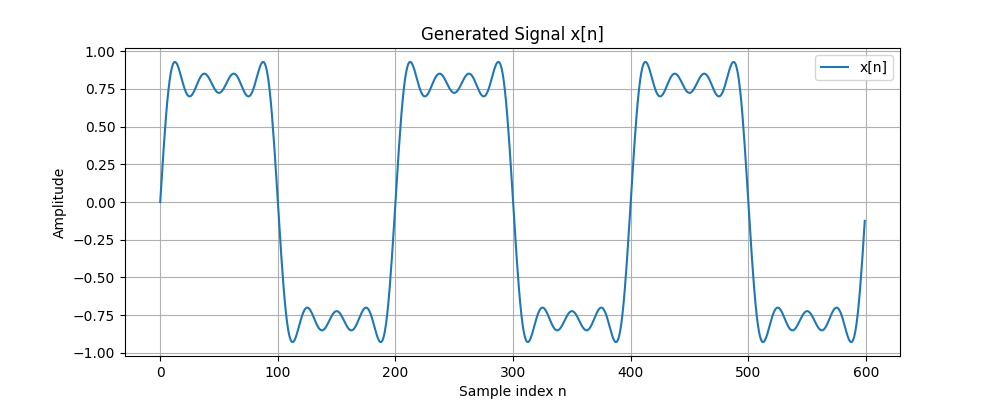
\includegraphics[width=0.8\textwidth]{fig/ex1_generated_signal.png}
    \caption{Generated Signal \( x[n] \)}
    \label{fig:ex1_generated_signal}
\end{figure}

\begin{figure}[h]
    \centering
    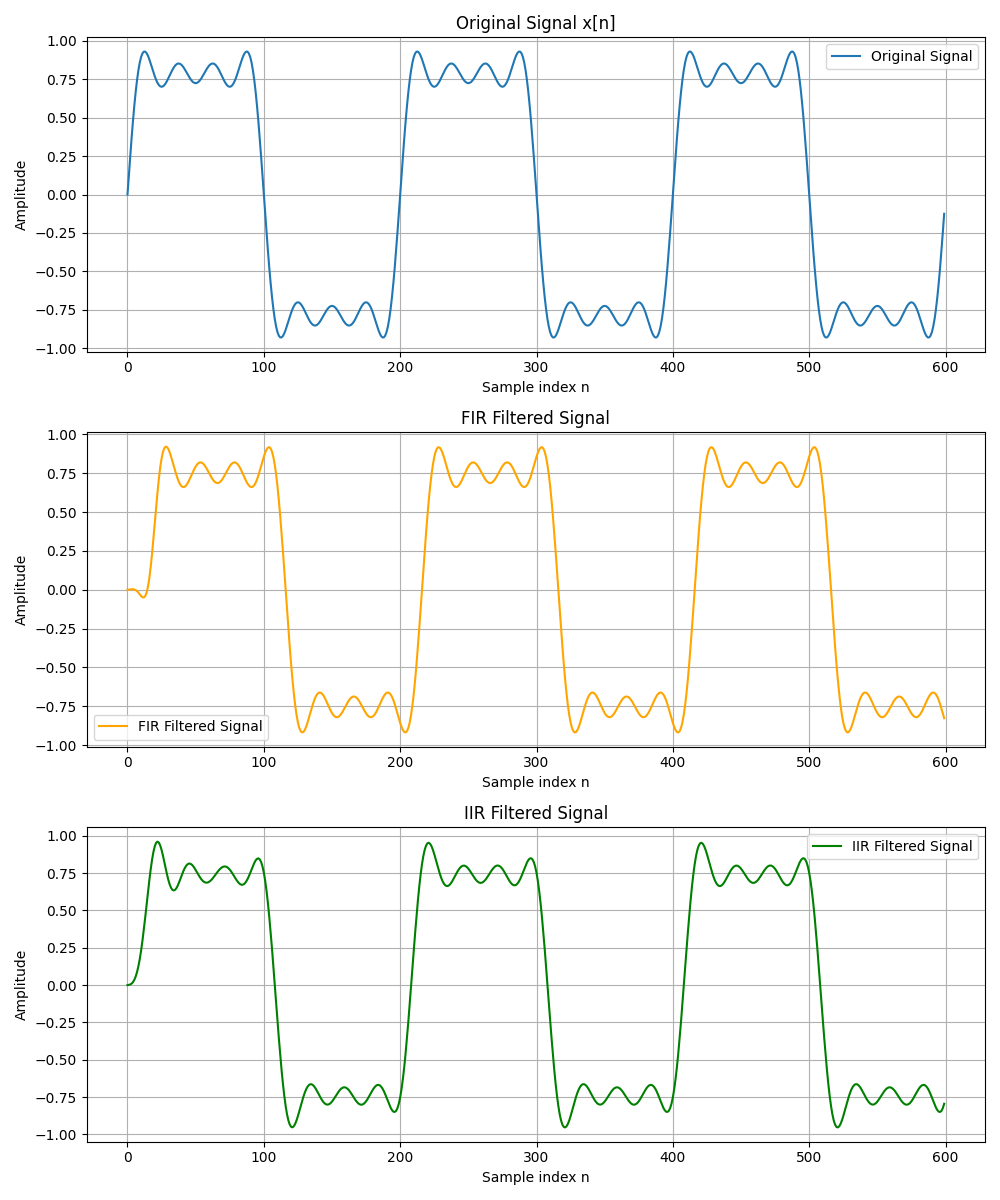
\includegraphics[width=0.8\textwidth]{fig/ex1_filtered_signals.png}
    \caption{Filtered Signals: FIR and IIR}
    \label{fig:ex1_filtered_signals}
\end{figure}

\subsection*{Conclusion}
The FIR and IIR filtered signals show how each filter type affects the original signal. FIR filters tend to introduce a uniform delay while preserving the waveform shape, whereas IIR filters can introduce phase distortions but achieve better magnitude response with a lower order.
